\chapter{Experimental Setup}

As our objective is to compare classical econometric methods to machine learning algorithms, we had to pick a real dataset with a binary variable of interest $y$. We also had to ensure that we had an adequate experimental setup that would allow us to implement the algorithms and experiment in a relatively flexible way, while also allowing us to record and analyse our results with relative ease.

\section{Database}
On the advice of our supervisors, we turned to the \textit{Enqu\^ete emploi en continu 2015} database \cite{enquete} from the INSEE website. \textit{Enqu\^ete Emploi} is the canonical database for the statistical system of knowledge of employment and unemployment in France, and one of the only sources that implements the definition of unemployment as defined by the International Labor Office \cite{ilo}.

The survey contains 431,678 observations taken in 2015, and provides original data on more than 100 variables, including occupation, female and youth activity, hours of work, precarious employment and wages. As such, using this data, we can better understand the situation of the unemployed as well as changes in the situation with regard to work: change from school to work, retirement activity, changes in occupation.

After downloading the dataset, we performed some basic manipulations to make it easier to work with (conversion from \texttt{DBF} to \texttt{SQLite} format), and then proceeded to create a "custom" subset of the database, such that we don't need to load all the data for each experiment, but only the parameters we are interested in. When these parameters were \textit{categorical}, we split them up into purely \textit{binary} variables to make our analyses easier.

\begin{figure}[!ht]
    \centering
    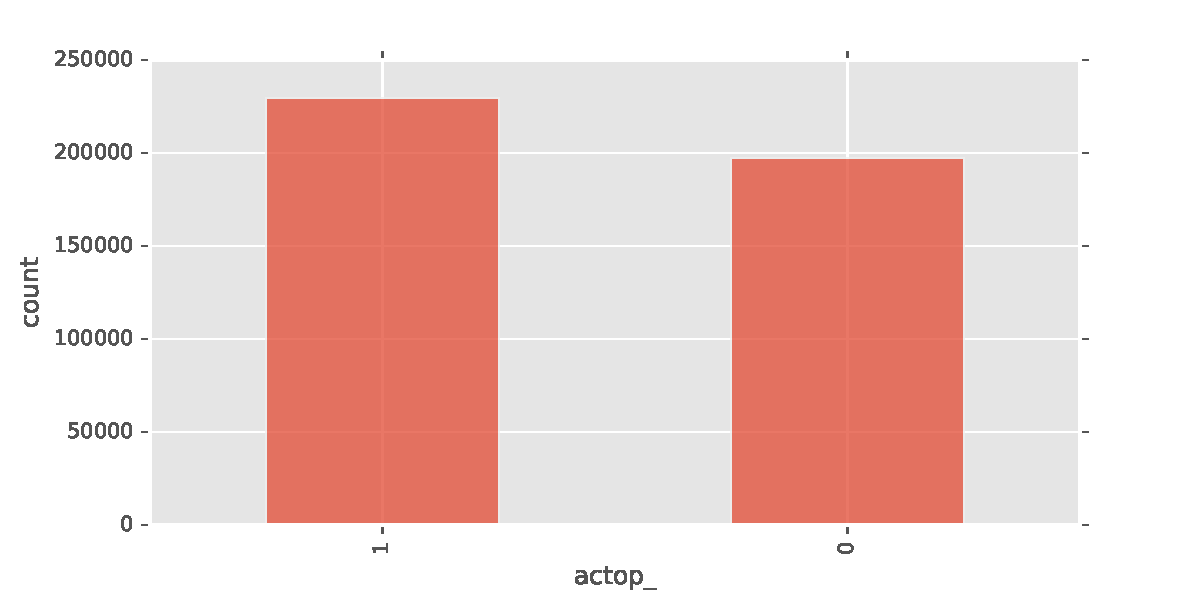
\includegraphics[width=0.8\textwidth]{img/database_actop_.pdf}
    \caption{Number of active (\texttt{actop\_=0}) and inactive (\texttt{actop\_=1}) persons}
    \label{fig:database_actop_}
\end{figure}

\section{Programming}
Our setup for programming, running and analysing the results of our experiments revolved around various tools that we have put in place:
\begin{itemize}
    \item The \texttt{Python} and \texttt{R} programming languages, along with the \texttt{scikit-learn} machine learning package \cite{python}\cite{R}\cite{learn}
    \item The \texttt{Git} source control manager \cite{git}, which enables us to keep track of different versions of our code (and thus project), while also letting us easily rollback changes, or run multiple versions of the code (e.g. with different parameters)
    \item \texttt{Jupyter} \cite{jupyter}, an interactive computing platform, which enables us to run code directly in the browser, and mix text with code snippets to document our work properly
\end{itemize}

When our experiments reached the point where computation on our personal laptops was too slow/not possible anymore, we turned to Amazon Web Services \cite{aws}, a cloud computing platform, which enabled us to provision very powerful machines almost immediately, and at a relatively small cost (\textasciitilde20\$ in total).

\section{Source}
All of our work and results can be found on the project's \href{https://github.com/ncocacola/econml/}{GitHub repository}\footnote{\texttt{https://github.com/ncocacola/econml/}} and in the
\href{https://github.com/ncocacola/econml/blob/master/econml.ipynb}{Jupyter Notebook}\footnote{\texttt{https://github.com/ncocacola/econml/blob/master/econml.ipynb}}.
